\section{Results} \label{sec_res}
\subsection{Fourier Analysis}
\begin{itemize}
\item vary $c$ and $S_n$
\item vary optical thickness and $S_n$
\item vary aspect ratio and $S_n$
\end{itemize}
\subsection{Numerical Results: Comparison of $CG$, $CG-SSOR$ and $CG-AMG$}
\begin{itemize}
\item homogeneous, rectangle with random point disturbances and arbitrary
polygons based on Triangle
\item iron-water, rectangle and arbitrary polygons with fake AMR
\end{itemize}
Pris de \cite{ml_guide}\\
\begin{description}
\item [Uncoupled:] Attempt to construct aggregates of optimal size ($3^d$
nodes in $d$ dimensions). Each process works independently and aggregates
cannot span processes.
\item [MIS:] Uses maximal independent set techniques \cite{mis} to define
aggregates. Aggregates can span processes. May provide better quality
aggregates than \bf{Uncoupled}, but computationally more expensive because it
requires matrix-matrix product.
\item[Symmetric Gauss-Seidel]
\item[Amesos-KLU:] Use \bf{KLU} through \bf{Amesos}. Coarse grid problem is
shipped to proc 0, solved and solution is broadcast.
\end{description}
The MultiLevelPreconditioner class provides default values for five different
preconditioner types, including classical smoothed aggregation for symmetric
positive definite or nearly symmetric definite systems.
\begin{description}
\item [option name:] SA
\item [max levels:] 10
\item [prec type:] V-cycle
\item [aggregation type:] Uncoupled-MIS
\item [aggregation dumping factor:] 4/3
\item [eigen-analysis type:] cg
\item [eigen-analysis iterations:] 10
\item [smoother sweeps:] 2
\item [smoother damping factor:] 1.0
\item [smoother pre or post:] both
\item [smoother type:] symmetric Gauss-Seidel
\item [coarse type:] Amesos-KLU
\item [coarse max size:] 128
\end{description}

\subsection{Homogeneous medium}
Medium: 10cm $times$ 10cm, cells: 100 $times$ 100, $S_8$,
Gauss-Legendre-Chebyshev, vacuum boundary condition, intensity of the source
1, $\Sigma_t =1$, $\Sigma_s=0.99$, SI solver, relative tolerance $10^{-8}$,
relative tolerance DSA $10^{-10}$.
\subsubsection{Quadrilateral cells}
Number of cells: 9990, number of dof: 39960
\begin{figure}[H]
\centering
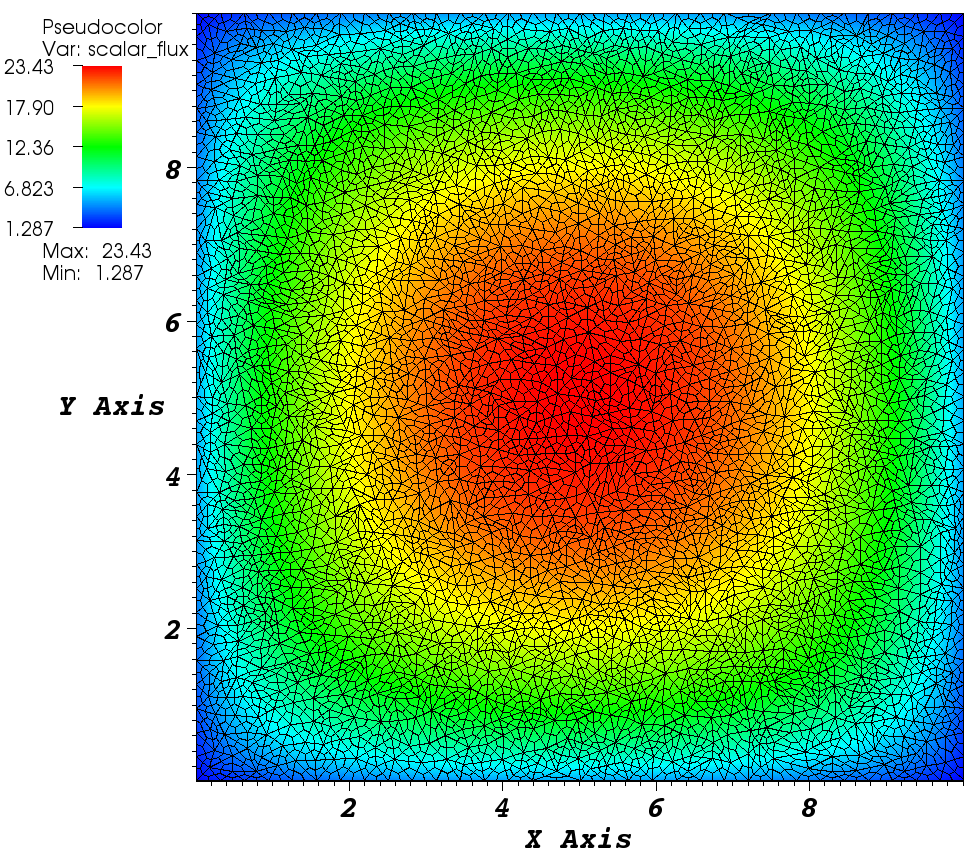
\includegraphics[width=0.8\textwidth]{homog_quad_crop}
\caption{Quadrilateral cells.}
\end{figure}
\begin{table}[H]
\begin{center}
\begin{tabular}{|c|c|c|c|c|c|c|}
\hline
 & No-DSA & CG & PCG-SGS & PSGS-ML-Uncoupled & PCG-ML-MIS & AGMG\\
\hline
SI iterations & 268 & 27 & 27 & 27 & 27 & 27 \\
Precond init (s) & NA & NA & 0.0142572 & 0.381872 & 1.21095 & 0.068\\
MIP calculation (s) & NA & 138.379 & 177.556 & 46.1957 & 44.7837 & 6.9311\\
CG iteration & NA & 35419 & 11414 & 729 & 702 & 674\\
Total calculation (s) & 309.395 & 172.181 & 211.933 & 80.1548 & 80.0387 &
40.827\\
\hline
\end{tabular}
\caption{Comparison of preconditioners with quadrilateral cells.}
\end{center}
\end{table}

\subsubsection{Polygonal cells}
Number of cells:16844, number of dof: 58442\\
\begin{description}
\item[Triangles:] 13654
\item[Quadrilaterals:] 250
\item[Pentagons:] 1400
\item[Hexagons:] 1306
\item[Heptagons:] 228
\item[Octagons:] 6
\end{description}
\begin{figure}[H]
\centering
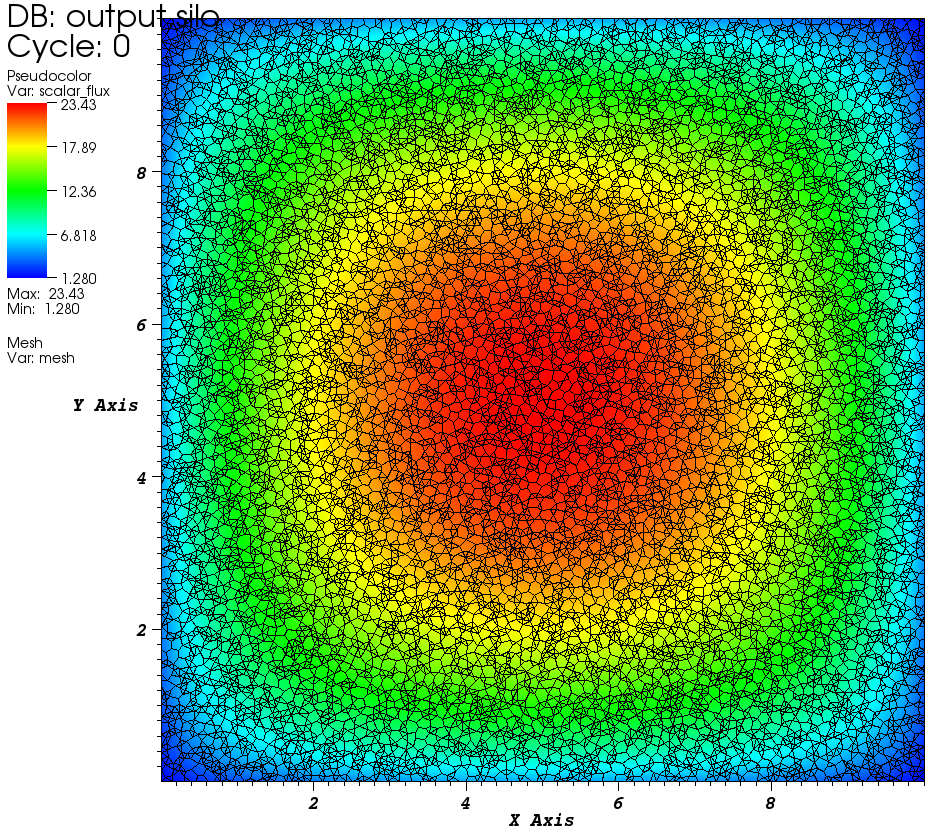
\includegraphics[width=0.8\textwidth]{homog_poly_crop}
\caption{Polygonal cells.}
\end{figure}
\begin{table}[H]
\begin{center}
\begin{tabular}{|c|c|c|c|c|c|c|}
\hline
 & No-DSA & CG & PCG-SGS & PSGS-ML-Uncoupled & PCG-ML-MIS & AGMG\\
\hline
SI iterations & 268 & 27 & 27 & 27 & 27 & 27\\
Precond init (s) & NA & NA & 0.0201421 & 0.482845 & 2.09054 & 0.097\\
MIP calculation (s) & NA & 210.128 & 303.423 & 78.0993 & 71.4493 & 11.0419\\
CG iteration & NA & 36352 & 13370 & 840 & 784 & 674\\
Total calculation (s) & 458.132 & 265.026 & 358.745 & 134.434 & 128.731 &
66.0207\\
\hline
\end{tabular}
\caption{Comparison of preconditioners with polygonal cells.}
\end{center}
\end{table}

\subsection{Hexagonal cells}
$S_{16}$, GLC, reflective boundary conditions, relative tolerance$ = 10^{-8}$,
MIP tolerance$ = 10^{-10}$
\begin{description}
\begin{figure}[H]
\centering
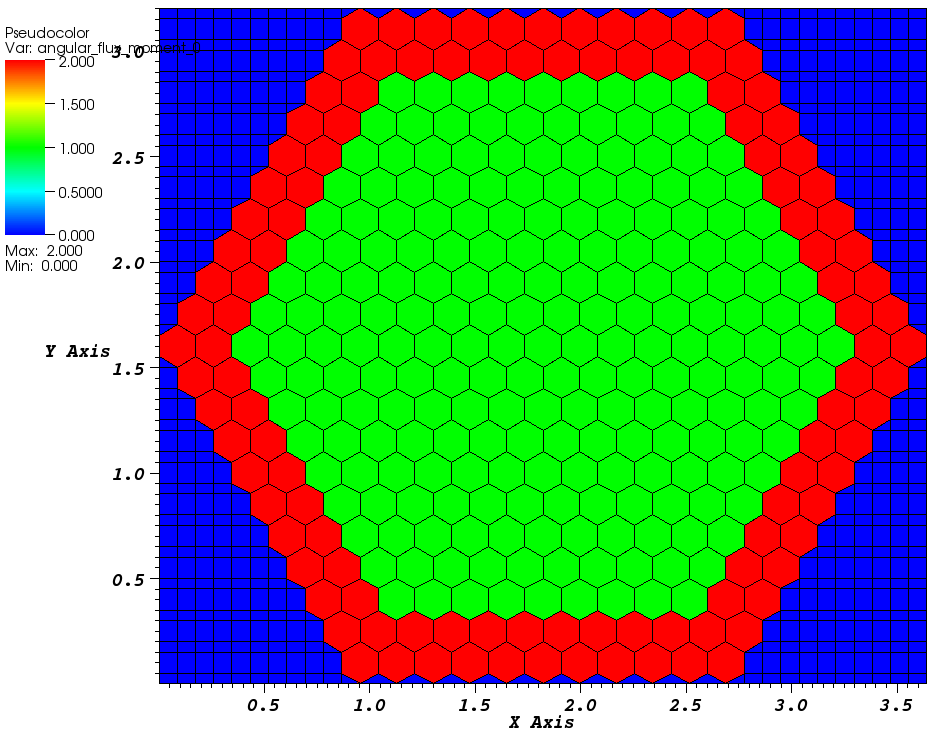
\includegraphics[width=0.8\textwidth]{source_crop}
\caption{Hexagonal cells.}
\end{figure}
\item[Green zone]: $\Sigma_t =1cm^{-1}$, $\Sigma_s = 0.9cm^{-1}$, source$ =
1cm^{-3}s^{-1}$
\item[Red zone]: $\Sigma_t = 1.5cm$, $\Sigma_s = 1.44cm^{-1}$, no source
\item[Blue zone]: $\Sigma_t = 1cm^{-1}$, $\Sigma_s = 0.3cm^{-1}$, no source
\end{description}
Number of cells: 835, number of dof: 3938
\begin{description}
\item[Triangles:] 64
\item[Quadrilaterals:] 440
\item[Hexagons:] 331
\end{description}
\begin{figure}[H]
\centering
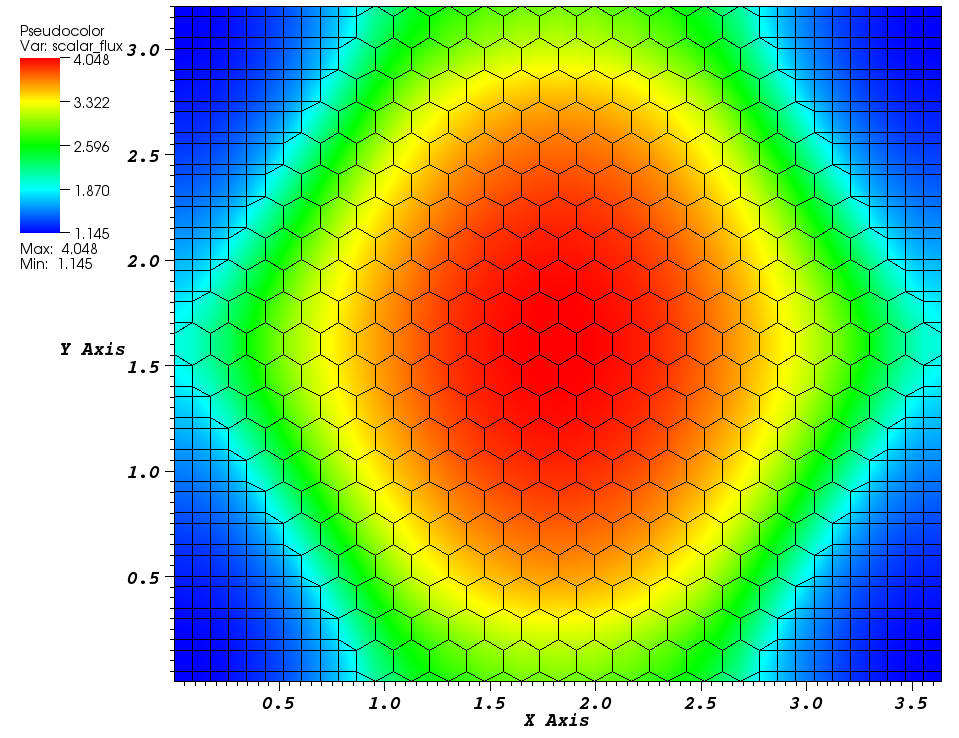
\includegraphics[width=0.8\textwidth]{heter_hexag_crop}
\caption{Hexagonal cells.}
\end{figure}
\begin{table}[H]
\begin{center}
\begin{tabular}{|c|c|c|c|c|c|c|}
\hline
 & No-DSA & CG & PCG-SGS & PSGS-ML-Uncoupled & PCG-ML-MIS & AGMG\\
\hline
SI iterations & 110 & 18 & 18 & 18 & 18 & 18\\
Precond init (s) & NA & NA &  0.00198889 & 0.049206 & 0.1407501 & 0.008\\
MIP calculation (s) & NA & 2.37668 & 5.98264 & 3.09196 & 3.00155 & 0.288559\\
CG iteration & NA & 4323 & 2747 & 355 & 341 & 245\\
Total calculation (s) & 30.7466 & 8.20233 & 11.5965 & 8.57338 & 8.67269 &
6.23169\\
\hline
\end{tabular}
\caption{Comparison of preconditioners with hexagonal cells.}
\end{center}
\end{table}
